% tcm.tex

\documentclass{standalone}
\usepackage{tikz}

\usetikzlibrary{shapes, positioning, arrows.meta, decorations.pathmorphing}

\begin{document}
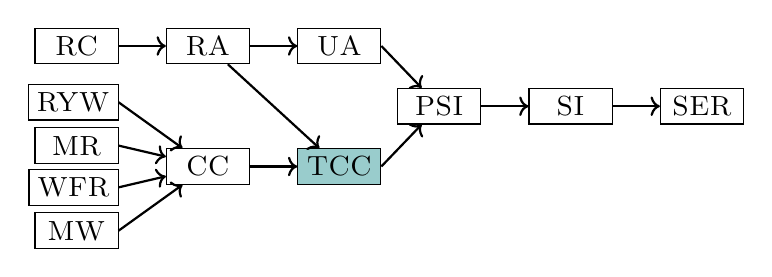
\begin{tikzpicture}[
	tcm/.style = {draw, rectangle,
	  inner sep = 3pt,
    minimum width = 30pt
    },
	]
  \node[tcm] (psi) {\textsc{PSI}};
  \node[tcm, right = 0.60cm of psi] (si) {\textsc{SI}};
  \node[tcm, right = 0.60cm of si] (ser) {\textsc{SER}};

  \node[tcm, above left = 0.30cm and 0.20cm of psi] (ua) {\textsc{UA}};
  \node[tcm, fill = teal!40, below left = 0.30cm and 0.20cm of psi] (tcc) {\textsc{TCC}};

  \node[tcm, left = 0.60cm of ua] (ra) {\textsc{RA}};
  \node[tcm, left = 0.60cm of tcc] (cc) {\textsc{CC}};

  \node[tcm, left = 0.60cm of ra] (rc) {\textsc{RC}};

  \node[tcm, above left = 0.35cm and 0.60cm of cc] (ryw) {\textsc{RYW}};
  \node[tcm, above left = -0.20cm and 0.60cm of cc] (mr) {\textsc{MR}};
  \node[tcm, below left = -0.20cm and 0.60cm of cc] (wfr) {\textsc{WFR}};
  \node[tcm, below left = 0.35cm and 0.60cm of cc] (mw) {\textsc{MW}};

  \path[->, thick]
    (rc) edge (ra)
    (ra) edge (ua)
    (ua.east) edge (psi)
    (psi) edge (si)
    (si) edge (ser)
    (cc) edge (tcc)
    (tcc.east) edge (psi)
    (ra) edge (tcc)
    (ryw.east) edge (cc)
    (mr.east) edge (cc)
    (wfr.east) edge (cc)
    (mw.east) edge (cc);
\end{tikzpicture}
\end{document}